\documentclass{article}%
\usepackage[T1]{fontenc}%
\usepackage[utf8]{inputenc}%
\usepackage{lmodern}%
\usepackage{textcomp}%
\usepackage{lastpage}%
\usepackage{graphicx}%
\usepackage{amsmath}%
%
\title{Homework 2}%
\author{Ann Kidder}%
\date{September 16, 2017}%
%
\begin{document}%
\normalsize%
\maketitle%
\section{Basic Concept Problems}%


\begin{figure}[h!]%
\centering%
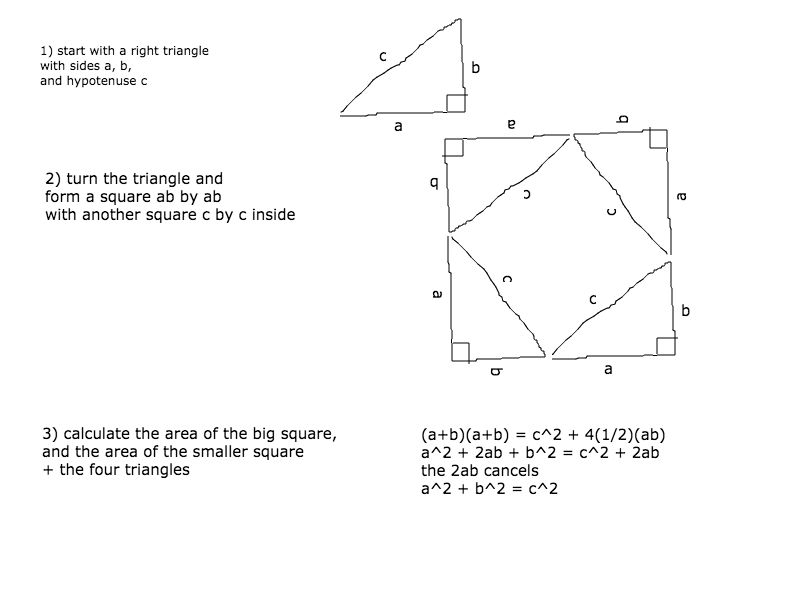
\includegraphics[width=350px]{pythagorean.jpg}%
\end{figure}

%


\begin{figure}[h!]%
\centering%
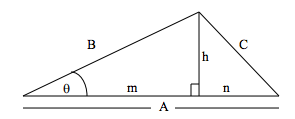
\includegraphics[width=100px]{triangle.jpg}%
\begin{alignat*}{2}%
&\textnormal{Given a triangle with sides A, B, and C }%
\textnormal{with height h and an angle } \theta\\%
& \textnormal{we know that the left triangle will}%
\textnormal{ have the property } m^2+h^2=B^2\\%
&\textnormal{and the right triangle will have the property }%
 h^2 + n^2 = C^2\\ &\textnormal{by the pythagorean theorem.}%
\textnormal{ Therefore:}\\%
&n = A - m\\%
&\textnormal{and } h^2 + (A-m)^2 = C^2\\%
&B^2-m^2+A^2-2Am+m^2 = C^2\\%
&\textnormal{Furthermore, we know } cos\theta = \frac{m}{B}\\%
&\textnormal{Therefore:}\\%
&B^2+A^2 -2ABcos\theta = C^2%
\end{alignat*}%
\end{figure}

%
\section*{9.3}%
\subsection*{20}%


\begin{figure}[h!]%
\centering%
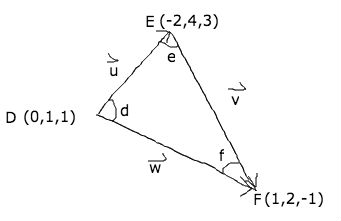
\includegraphics[width=150px]{tri2.jpg}%
\begin{alignat*}{2}%
\vec{u} &= <-2,3,2>\\%
\vec{v} &= <3,-2,-4>\\%
\vec{w} &= <1,1,-2>\\%
\textnormal{The angle at D:} \\%
<-2,3,2>\cdot<1,1,-2> &=\|<-2,3,2>\| \|<1,1,-2>\|cosd\\%
-3 &= \sqrt{17}\sqrt{6}cosd\\%
cos^-1(\frac{-3}{\sqrt{102}}) &= d\\%
d & \approx{107.28}^\circ\\%
\textnormal{The angle at E:} \\%
-(<-2,3,2>)\cdot<3,-2,-4> &=\|<-2,3,2>\| \|<3,-2,-4>\|cose\\%
20 &= \sqrt{17}\sqrt{29}cose\\%
cos^-1(\frac{20}{\sqrt{493}}) &= e\\%
e & \approx{25.74}^\circ\\%
\textnormal{The angle at F:} \\%
-(<1,1,-2>)\cdot-(<3,-2,-4>) &=\|<1,1,-2>\| \|<3,-2,-4>\|cosf\\%
9 &= \sqrt{6}\sqrt{29}cosf\\%
cos^-1(\frac{9}{\sqrt{174}}) &= f\\%
f & \approx{46.98}^\circ\\%
\end{alignat*}%
\end{figure}

%
\subsection*{30}%
\begin{alignat*}{2}%
\|a\| &= \sqrt{5}\\%
comp_a b &= \frac{a \cdot b}{\|a\|} = \frac{-4+2}{\sqrt{5}} = \frac{-2}{\sqrt{5}}\\%
\textnormal{The vector projection is:}\\%
proj_a b &= \frac{-2}{\sqrt{5}}\frac{<1,2>}{\sqrt{5}} = \frac{-2}{5} <1,2>\\%
proj_a b &= <\frac{-2}{5}, \frac{-4}{5}>%
\end{alignat*}

%
\subsection*{31}%
\begin{alignat*}{2}%
a = <2,-1,4> & \textnormal{ and } b = <0,1,\frac{1}{2}>\\%
\| a \| &= \sqrt{4+1+16} = \sqrt{21}\\%
comp_a b &= \frac{a \cdot b}{\sqrt{21}} = \frac{1}{\sqrt{21}}\\%
\textnormal{The vector projection is:}\\%
proj_a b &= \frac{1}{\sqrt{21}}\frac{<2,-1,4>}{\sqrt{21}} = \frac{1}{21}<2,-1,4>\\%
proj_a b &= <\frac{2}{21},\frac{-1}{21},\frac{4}{21}>\\%
\end{alignat*}

%
\subsection*{43}%
\begin{alignat*}{2}%
\intertext{Let all sides of the cube be length = 1, and let the edges lie along the x, y, z axis}\\%
\text{The diagonal vector, }\vec{d}\text{ from (0,0,0) to (1,1,1) = <1,1,1>}\\%
\text{Let the unit vector } \vec{k} = <0,0,1> \text{be a side.}\\%
\text{The angle between } \vec{d} \text{ and } \vec{k} \text{ is:}\\%
cos\theta &= \frac{<0,0,1> \cdot <1,1,1>}{\|u\|\|v\|}\\%
&= \frac{0+0+1}{\sqrt{1}\sqrt{3}}\\%
&= \frac{1}{\sqrt{3}} \\%
\theta &= cos^-1 \frac{1}{\sqrt{3}}\\%
&= 54.74^\circ%
\end{alignat*}

%
\subsection*{46}%


\begin{figure}[h!]%
\centering%
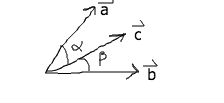
\includegraphics[width=150px]{ang1.jpg}%
\end{figure}

%
\begin{alignat*}{2}%
cos\alpha &= \frac{a \cdot c}{\|a\| \|c\|}\\%
&= \frac{a \cdot (\|a\|b+\|b\|a))}{\|a\| \|c\|}\\%
&= \frac{a \cdot \|a\|a \cdot b + \|b\|a \cdot a}{\|a\| \|c\|}\\%
&= \frac{\|a\|a \cdot b + \|b\| \|a\|^2}{\|a\| \|c\|}\\%
&= \frac{a \cdot b + \|b\| \|a\|}{\|c\|}\\%
cos\beta &= \frac{b \cdot c}{\|b\| \|c\|}\\%
&= \frac{b \cdot (\|a\|b+\|b\|a))}{\|b\| \|c\|}\\%
&= \frac{\|a\| b \cdot b + \|b\|a \cdot b}{\|b\| \|c\|}\\%
&= \frac{\|a\| \|b\|^2 + \|b\| a \cdot b}{\|b\| \|c\|}\\%
&= \frac{\|a\| \|b\| + a \cdot b}{\|c\|}\\%
\textnormal{Now we can see that } cos \alpha = cos \beta\\%
 \frac{a \cdot b + \|b\| \|a\|}{\|c\|} &= \frac{\|a\| \|b\| + a \cdot b}{\|c\|}\\%
\end{alignat*}

%
\section*{9.4}%
\subsection*{20}%
\begin{alignat*}{2}%
\intertext{The cross product is orthogonol to both i+j+k and 2i+k:}\\%
i+j+k = <1,1,1> & \textnormal{ and } 2i+k = <2,0,1>\\%
<1,1,1>\times <2,0,1> &= (1-0) \vec{i}+(2-1) \vec{j}+(0-2) \vec{k}\\%
<1,1,1>\times <2,0,1> &= <1,1,-2>\\%
\intertext{Divide by the magnitude to find the unit vector:}\\%
\textnormal{unit vector } &= \frac{<1,1,-2>}{\sqrt{1+1+4}}\\%
&= <\frac{1}{\sqrt{6}},\frac{1}{\sqrt{6}},\frac{-2}{\sqrt{6}}>\\%
\intertext{The second unit vector would be the negative of the first:}\\%
&= <\frac{-1}{\sqrt{6}},\frac{-1}{\sqrt{6}},\frac{2}{\sqrt{6}}>\\%
\end{alignat*}

%
\subsection*{22}%


\begin{figure}[h!]%
\centering%
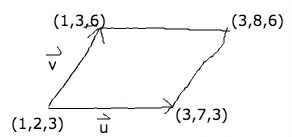
\includegraphics[width=150px]{para1.jpg}%
\end{figure}

%
\begin{alignat*}{2}%
\vec{u} = <2,5,0> \textnormal{ and } \vec{v} = <0,1,3>\\%
A &= \|<2,5,0> \times <0,1,3>\| \\%
A &= \|<-15,6,-2>\| \\%
A &= \sqrt{265}%
\end{alignat*}

%
\subsection*{24}%
\subsection*{a)}%
\begin{alignat*}{2}%
\vec{PQ} = <1,2,1> \textnormal{ and } \vec{PR} = <5,0,-2>\\%
\textnormal{The vector orthogonol to the plane = } \vec{PQ} \times \vec{PR}\\%
\vec{PQ} \times \vec{PR} = <-5,7,-10>\\%
\end{alignat*}

%
\subsection*{b)}%
\begin{alignat*}{2}%
A &= \frac{\|<-5,7,-10>\|}{2}\\%
A &= \frac{\sqrt{174}}{2} \approx 6.6%
\end{alignat*}

%
\subsection*{33}%
\subsection*{a)}%
\begin{alignat*}{2}%
d &= \|b\|sin\theta\\%
&=\frac{\|a\|}{\|a\|}\|b\|sin\theta\\%
&= \frac{\|a\|\|b\|sin\theta}{\|a\|}\\%
&= \frac{\|a \times b\|}{\|a\|}\\%
\end{alignat*}

%
\subsection*{b)}%
\begin{alignat*}{2}%
\vec{a} = <-1,-2,-1> \textnormal{ and } \vec{b} = <1, -5, -7>\\%
d &= \frac{\|<-1,-2,-1> \times <1, -5, -7>\|}{\sqrt{1+4+1}}\\%
&= \frac{\|<9,-15,7>\|}{\sqrt{6}}\\%
&= \frac{\sqrt{355}}{\sqrt{6}}\\%
d & \approx 7.69\\%
\end{alignat*}

%
\section*{9.5}%
\subsection*{2}%
\begin{alignat*}{2}%
\textnormal{vector equation } &= <6,-5,2> + t<1,3,\frac{-2}{3}>\\%
&= <6+t, -5+3t, 2+\frac{-2}{3}t>\\%
\textnormal{The parametric equations are:}\\%
x(t) &= 6+t\\%
y(t) &= -5+3t\\%
z(t) &= 2+\frac{-2}{3}t\\%
\end{alignat*}

%
\subsection*{5}%
\begin{alignat*}{2}%
x(t) &= 1+t\\%
y(t) &= 3t\\%
z(t) &= 6+t\\%
\end{alignat*}

%
\subsection*{10}%
\begin{alignat*}{2}%
\vec{n_1} = <1,2,3> \textnormal{ and } \vec{n_2} = <1,-1,1>\\%
<1,2,3> \times <1,-1,1> \textnormal{is a line parallel to the line of intersection.}\\%
<1,2,3> \times <1,-1,1> = <5,2,-3>\\%
\textnormal{Plug in z=0 to solve x, y and find a point on the line of intersection}\\%
x+2y=1 \textnormal{ and } x-y &=1\\%
\textnormal{This gives us } 3y &= 0 \\%
\textnormal{Therefore (1,0,0) lies on the line of intersection and the symmetric equations are:}\\%
\frac{x-1}{5} &= \frac{y}{2} = \frac{-z}{3}\\%
\textnormal{And the parametric equations are:}\\%
x(t) &= 1+5t\\%
y(t) &= 2t\\%
z(t) &= -3t\\%
\end{alignat*}

%
\subsection*{18}%
\begin{alignat*}{2}%
\textnormal{Check ratio of coefficients to test if parallel:}\\%
\frac{1}{-1} = \frac{3}{1} = \frac{-1}{3}\\%
-1 \neq 3 \neq -3 \textnormal{therefore the lines are NOT parallel}\\%
\textnormal{Solve system of equations to test if intersecting:}\\%
1 +2t &= -1+s\\%
3t &= 4+s\\%
2-t &= 1+3s\\%
\textnormal{Solve the first equation for t:}\\%
2t &=-2+s\\%
t &= -1 + \frac{s}{2}\\%
\textnormal{Plug into the second equation:}\\%
3(-1+\frac{s}{2}) = 4+s\\%
-3+\frac{3s}{2} = 4+s\\%
\frac{s}{2} = 7\\%
s = 14\\%
\textnormal{Plug s=14 this into the equation for t:}\\%
t=-1+\frac{14}{2} = -6\\%
\textnormal{Plug s=14 and t=-6 into the third equation:}\\%
2+-6 = 1+3(14)\\%
-4 \neq 43 \textnormal{therefore the lines do not intersect.}\\%
\textnormal{Since the lines are not parallel and do not intersect, they must be skew.}\\%
\end{alignat*}

%
\subsection*{25}%
\begin{alignat*}{2}%
P(0,1,1) \textnormal{ and }Q(1,0,1) \textnormal{ and }R(1,1,0)\\%
\vec{PQ} = <1-0,0-1,1-1> &= <1,-1,0>\\%
\vec{PR} = <1-0,1-1,0-1> &= <1,0,-1>\\%
\textnormal{Take the cross product to get the coefficients of the plane equation:}\\%
<1,-1,0> \times <1,0,-1> = <1,1,1> \\%
\textnormal{Use P as the point for the equation of the plane:}\\%
1(x-0)+1(y-1)+1(z-1) &= 0\\%
x+y+z &=2\\%
\end{alignat*}

%
\subsection*{27}%
\begin{alignat*}{2}%
\textnormal{The points P(6,0,-2) and Q(4,3,7) are on the plane.}\\%
\textnormal{Set t=1 to get a third point on the plane, R(2,8,11)}\\%
\vec{PQ} = <4-6,3-0,7-(-2)> = <-2,3,9>\\%
\vec{PR} = <2-6,8-0,11-(-2)> = <-4,8,13>\\%
\textnormal{Take the cross product to get the coefficients of the plane equation:}\\%
<-2,3,9> \times <-4,8,13> = <-33,-10,-4>\\%
\textnormal{Use P as the point for the equation of the plane:}\\%
-33(x-6)+-10(y-0)+-4(z+2) &= 0\\%
-33x+198-10y-4z-8 &= 0\\%
-33x-10y-4z &= -190%
\end{alignat*}

%
\subsection*{32}%
\begin{alignat*}{2}%
\textnormal{Let Q be the plane that we are looking for.}\\%
\textnormal{Set z=0 to get a point on the line of intersection:}\\%
(1,3,0)\\%
\textnormal{To get a normal vector for Q, take the cross product of two vectors parallel to Q.}\\%
\textnormal{The normal vector of the plane perpendicular to Q is parallel to Q:}\\%
<1,1,-2>\\%
\textnormal{Get a second vector parallel to Q by taking the cross product of the normal vectors }\\%
\textnormal{of the two planes that form the line of intersection that Q passes through.}\\%
<1,0,-1> \times <0,1,2> &= <1,-2,1>\\%
\textnormal{Now take the cross product of these two vectors:}\\%
<1,1,-2> \times <1,-2,1> &= <-3,-3,-3>\\%
\textnormal{Plug these into the plane equation:}\\%
-3(x-1)-3(y-3)-3(z-0) &= 0\\%
-3x+3-3y+9-3z &= 0\\%
-3x-3y-3z &= -12\\%
-3(x+y+z) &= -12\\%
x+y+z &= 4\\%
\end{alignat*}

%
\subsection*{56}%
\begin{alignat*}{2}%
d &= \frac{|1(6)+(-2)(0)+(-4)(-2) + (-8)|}{\sqrt{1^2+(-2)^2+(-4)^2}}\\%
&= \frac{|6+8-8|}{\sqrt{21}}\\%
&= \frac{6}{\sqrt{21}}\\ %
d &\approx 1.31\\%
\end{alignat*}

%
\subsection*{58}%
\begin{alignat*}{2}%
\textnormal{To find the distance we need a point on one plane.}\\%
\textnormal{Plug in z=0 to the first equation.}\\%
0 &= 4y - 2x\\%
y &= \frac{1}{2}x\\%
\textnormal{Therefore the point (2,1,0) is on the first plane.}\\%
\textnormal{Now we can use the distance formula.}\\%
d &= \frac{|3(2) + -6(1) + 9(0) + -1|}{\sqrt{3^2+(-6)^2+9^2}}\\%
&= \frac{|6-6-1|}{\sqrt{126}}\\%
&= \frac{1}{\sqrt{126}}\\%
d & \approx .09\\%
\end{alignat*}

%
\end{document}